\documentclass{article}

\usepackage{graphicx,multicol}

\author{Patrick Daley}
\title{Validation of 2-Site Program}

\addtolength{\oddsidemargin}{-.875in}
\addtolength{\evensidemargin}{-.875in}
\addtolength{\textwidth}{1.75in}
\addtolength{\topmargin}{-.875in}
\addtolength{\textheight}{1.75in}

\begin{document}

\maketitle

This document outlines the validation process for the 2-site program. Each section describes a test we have run on the code to ensure the results can be trusted. They are mostly cases with certain parameters set to zero so that we can compare the results of the program to the known results at that limit. 

\section{Atomic Limit with no Interactions}
The program was run with the hoping (t) and the on-site interactions (U) set to zero and performed at half filling. In this case we expect the DOS to be a rectangle with edges at -W/2 and W/2 (W is the disorder strength). We expect this since when there are no onsite interactions the energies of the contributions should be the eigenvalues of the single electron hamiltonian. There are no off diagonal terms (no hoping) so the contribution energies should just be the site potentials and they are chosen from a uniform distribution bounded between -W/2 and W/2. The GIPR should be 1 between -W/2 and W/2 and then 0.5 everywhere else.

The graphs outputted from the program look precisely as we expected.  The DOS for one case is shown in figure 1. Unfortunately the GIPR had NAN (not a number) for $ | frequency | > W/2 $ because of divisions by zero but the values within the range were all 1 as expected. This data couldn't be graphed but can be viewed in the file dos2\_t0u0w0.dat in the \textit{data} folder.

\begin{center}
	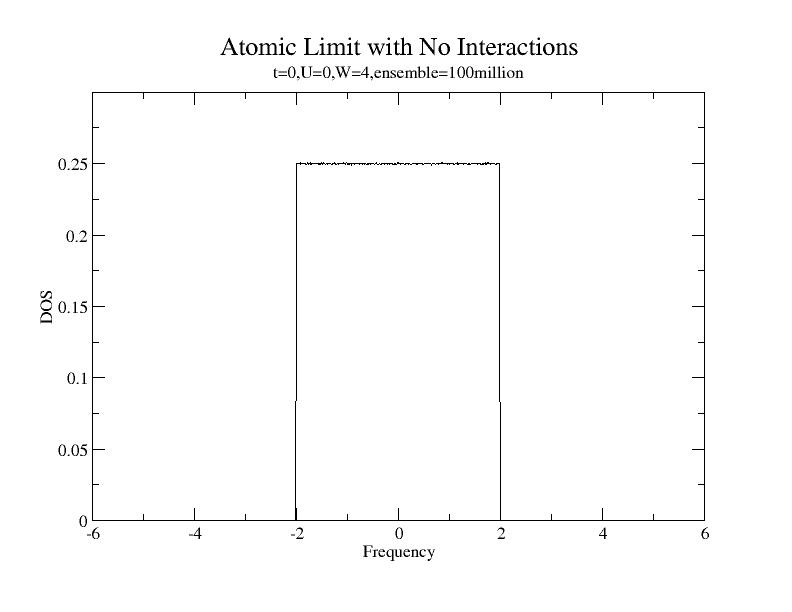
\includegraphics[width=250px]{dos2_t0u0w4.jpg} \\
	Figure 1: The DOS for the non interacting case with no hoping.
\end{center}



\section{Atomic Limit with Interactions}
The program was run with the hoping (t) set to zero but with the on-site interactions (U) not set to zero.

\begin{center}
	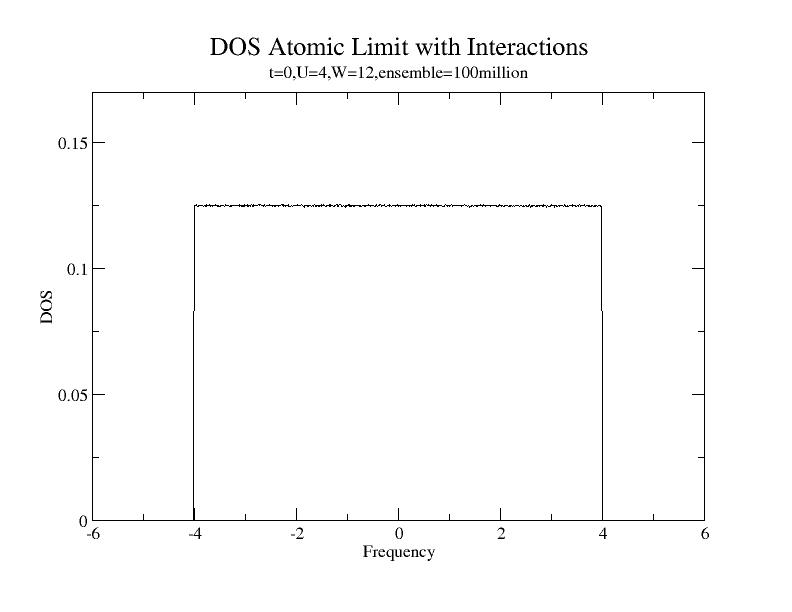
\includegraphics[width=250px]{dos2_t0u4w12.jpg} \\
	Figure 2: The DOS for the interacting case with no hoping.
\end{center}

\section{Non Interacting Case}
The program was run with hoping (t) but with the on-site interactions (U) set to zero. In this case can compare the data to another code that solves the problem when there are no interactions (noint2.f90) as well as published work by Johri and Bhatt[1]. The non-interacting code (noint2.f90) was run with same parameters as main.f90 and the random number generator used to assign site potentials were both seeded with the same constant so the two graphs should be identical. This is the case and is shown in figure \ref{noint}.
\begin{center} 
	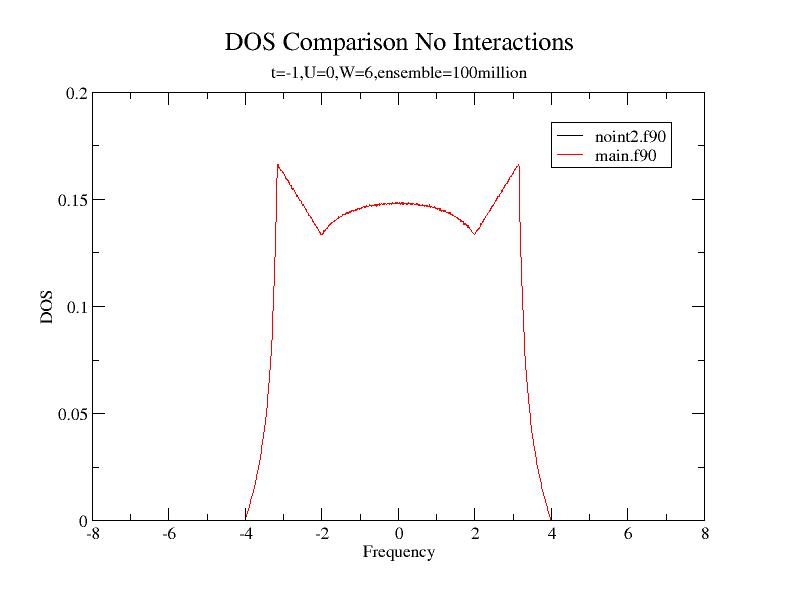
\includegraphics[width=250px]{dos_compareu0.jpg} \\ \label{noint}
	Figure \ref{noint}: The DOS for the non interacting case with hoping.
\end{center}
The the non-interacting code does output the GIPR however both the graphs can be compared to those published in Johri and Bhatt's paper.
\section{Comparison with Published Results}
The program is run at 
\section{Symmetry away from Half Filling}
The program is run with hoping (t/=0) and onsite interactions(U/=0) away from half filling (mu/=$\frac{U}{2}$). There is little published work at the moment for this simulation and it is impossible to calculate analytically however the DOS and GIPR for a filling of $0.5-n$ should be the reflection about the y axis of the DOS and GIPR with filling $0.5+n$.
\begin{center}
	\line(1,0){400}
\end{center}
[1] S. Johri and R. Bhatt, Physical Review Letters \textbf{109}, 076402 (2012). \newline
[2] J. Perera and R. Wortis,
\end{document}